%%%%%%%%%%%%%%%%%%%%%%%%%%%%%%%%%%%%%%%%%%%%%%%%%%%%%%%%
%
% Change the option between square brackets
% depending on the document you have to write:
%
% proposal    for the initial proposal
% review      for the literature review
% progress    for the progress report
% final       for the final report
% 
%%%%%%%%%%%%%%%%%%%%%%%%%%%%%%%%%%%%%%%%%%%%%%%%%%%%%%%%
\documentclass[proposal]{cmpreport}
\makeatletter
\input{t1pcr.fd}
\makeatother
\setlength{\footnotesep}{3ex}

% Some package I am using. You may not need them
%
\usepackage{rotating}
\usepackage{subfloat}

%\setkeys{Gin}{draft}

%%%%%%%%%%%%%%%%%%%%%%%%%%%%%%%%%%%%%%%%%%%%%%%%%%%%%%%%
%
%  Fill in the fields with:
%
%  your project title
%  your name
%  your registration number
%  your supervisor's name
%
%%%%%%%%%%%%%%%%%%%%%%%%%%%%%%%%%%%%%%%%%%%%%%%%%%%%%%%%
\title{Study Of AI Algorithms For The Solution Of Puzzles With Minimum Number Of Moves}

%%%%%%%%%%%%%%%%%%%%%%%%%%%%%%%%%%%%%%%%%%%%%%%%%%%%%%%%
%
% The author's name is ignored if the following command 
% is not present in the document
%
% Before submitting a PDF of your final report to the 
% project database you may comment out the command
% if you are worried about lack of anonimity.
%
%%%%%%%%%%%%%%%%%%%%%%%%%%%%%%%%%%%%%%%%%%%%%%%%%%%%%%%%
\author{Luke Garrigan}


\registration{100086495}
\supervisor{Dr Pierre Chardaire}
%%%%%%%%%%%%%%%%%%%%%%%%%%%%%%%%%%%%%%%%%%%%%%%%%%%%%%%%
%
% Fill in the field with your module code.
% this should be:
%
% for BIS            -> CMP-6012Y
% for BUSINESS STATS -> CMP-6028Y
% for other students -> CMP-6013Y
%
%%%%%%%%%%%%%%%%%%%%%%%%%%%%%%%%%%%%%%%%%%%%%%%%%%%%%%%%
\ccode{CMP-6012Y}

%%%%%%%%%%%%%%%%%%%%%%%%%%%%%%%%%%%%%%%%%%%%%%%%%%%%%%%%%%%%%%%%%%
%
% If you do not want a list of figures and a list of tables
% to appear after the table of content then uncomment this line 
%
% Note that the class file contains code to avoid
% producing an empty list section (e.g list of figures) if the 
% list is empty (i.e. no figure in document).
%
% The command also prevents inserting a list of figures or tables 
% anywhere else in the document
%
% Some supervisors think that a report should not contain these
% lists. Please ask your supervisor's opinion.
%
%%%%%%%%%%%%%%%%%%%%%%%%%%%%%%%%%%%%%%%%%%%%%%%%%%%%%%%%%%%%%%%%%%
%\nolist,

%%%%%%%%%%%%%%%%%%%%%%%%%%%%%%%%%%%%%%%%%%%%%%%%%%%%%%%%%%%%%%%%%%
%
% Comment out if you want your list of figures and list of
% tables on two or more pages, in particular if the lists do not fit 
% on a single page.
%
%%%%%%%%%%%%%%%%%%%%%%%%%%%%%%%%%%%%%%%%%%%%%%%%%%%%%%%%%%%%%%%%%%
\onePageLists

\begin{document}


\section{Introduction}




The goal of this project is to design, implement and compare algorithms for solving puzzles such as the sliding-tile and Rubik's Cube in the minimum number of moves. I will be implementing Dijkstra's single-source shortest-path which is an algorithm used to find shortest paths from one
given vertex to all other vertices in a non-negatively weighted graph. An example for this algorithm could be represented in road networks \cite{DBLP:journals/afp/NordhoffL12}.

I will be designing the A* algorithm and analyse its applicability with its exponential growth \cite{DBLP:journals/ai/Korf93}. The A* algorithm is widely used for path-finding and graph traversal, the course of plotting and efficiently traversing paths between nodes.

The iterative deepening A* algorithm is my main focus, it is also a graph traversal and path search algorithm with the goal to find the shortest path between nodes. IDA* is a depth-first search algorithm thus its memory usage is lower than A*, however it doesn't use dynamic programming thus often ends up exploring the same nodes multiple times. I will be analysing and comparing it with the A* with Recursive Best First Search algorithm. RBFS is a recurisve algorithm in which attempts to mimic the operations of A* search, however it executes using a linear space rather than A*'s exponential space complexity. RBFS uses an evaluation limit to prevent it continually going down a specific path \cite{DBLP:conf/aaai/HatemKR15}.

I will also incorporate and test alternative algorithms such as Memory Bounded A*, which is a shortest path algorithm based on A* with the main advantage of using bounded memory while the A* algorithm utilises exponential memory. I will additionally produce my own personal solutions and methods.

I will be implementing the algorithms in Java as I have years of experience java programming, from developing my own games with built in artificial intelligence to path finding using the A* search algorithm for finding the shortest path.  


\section{The Sliding Tile Puzzle} \label{sec1}

\begin{figure}[ht]
	\centering
	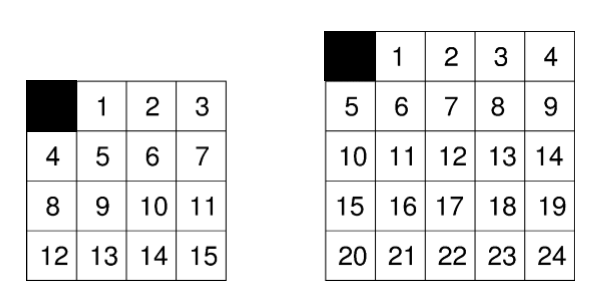
\includegraphics[width=0.5\textwidth]{sliding_tile}
	\captionsetup{justification=centering}
	\caption{The goal states of the Fifteen and Twenty-Four Puzzles}
\end{figure}

	In the Sliding tile Puzzle any tile which is horizontally or vertically adjacent to the blank tile can be repositioned into that empty space. The goal of the puzzle is to move the tiles from a set composition to the goal state as shown in Figure 1. The main objective is to reach the target state in a minimum number of moves. 
	
	I will be focusing on the 4x4 and 5x5 sliding puzzles because they require a heuristic search algorithm such as A*, whereas a 3x3 sliding puzzle could be solved with brute force as it only has a total of 181,440 states and can be solved optimally with a breadth-first search \cite{DBLP:journals/ai/KorfF02}. I will be testing and evaluating different types of heuristics for this given problem starting off with the Manhattan distance. The Manhattan distance is The distance between two points in a grid, based on a strictly horizontal and/or vertical path. The Manhattan distance is the simple sum of the horizontal and vertical components.
	
	I will be testing the linear-conflict heuristic which has a significant improvement over the Manhattan distance, as it considers the goal row or column, but reversed relative to each other. What this means is that two tiles \verb/X/ and \verb/Y/ are in linear conflict if \verb/X/ and \verb/Y/ are in the same line as well as the goal positions, \verb/Y/ is to the left of \verb/X/ and goal position of \verb/Y/ is to the right of goal position of \verb/X/. Both the linear-conflict heuristic and Manhattan heuristic are admissible meaning they don't overestimate the cost of reaching the goal. 





\section{The Rubiks Cube} \label{sec2}
\begin{figure}[ht]
	\centering
	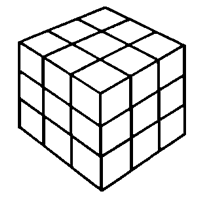
\includegraphics[width=0.3\textwidth]{rubiks}
	\captionsetup{justification=centering}
	\caption{The Rubik's Cube}
\end{figure}
The Rubik's Cube is the worlds best known combinatorial puzzle. Each 3x3 plane can be rotated 90 or 180 
degrees, clockwise or anticlockwise. The goal of the game is to have all 6 sides showing only one colour. The 3x3x3 Rubik's Cube contains about 4.3252x1019 different reachable states.


There are 20 movable subcubes, or cubies, which can be divided into eight corner cubies, with three faces each, and twelve edge cubies, with two faces each.
There are 88,179,840 different positions and orientations of the corner cubies, and the number of moves needed to solve just the corner cubies ranges from
zero to eleven.\cite{DBLP:journals/ai/KorfF02}

My goal is to implement the IDA* algorithm which will solve the Rubik's cube in a minimum number of moves in the best possible time. Richard E. Korf predicted the Time complexity of iterative-deepening-A* algorithm for the Rubik's cube within 1\% accuracy in every case. \cite{DBLP:journals/ai/KorfRE01}

\clearpage



\section{Risk Analysis} \label{sec2}
The main risks which I face in tackling this project are based primarily around the time allocated. I have many algorithms which I want to design, implement and experiment for both the sliding tile puzzle and the Rubik's Cube, that I may run into trouble with time and struggle to finish certain algorithms. I have prepared for this and set out a priority ordered list for the algorithms which I will develop based upon. As shown by the Gantt Chart I have allocated the main algorithms a time slot in which they share with the lesser priority algorithms, this method will allow for completion of higher priority algorithms before beginning development of lower priority ones as shown in Table 1. 

\begin{table}[ht]
	\caption{Algorithm Priority Table}
	\begin{center}
		\begin{tabular}{clr} \hline
			Algorithm & Sliding Tile & Rubiks Cube \\ \hline
			Iterative deepening A*  & 1 & 1 \\
			Single-source shortest-path & 3 & 3 \\ 
			A* with Recursive Best First Search & 2 & 2 \\ 
			Memory Bounded A* & 3 & 3 \\ \hline
		\end{tabular}
	\end{center}
\end{table}

In developing this prioritisation system I should be able to get the core components necessary for analysis and testing. I am focusing primarily on the algorithms which have been proved to have the best outcome in terms of completing the puzzles in the minimum number of moves and computing cost. With the guidelines set in terms of prioritisation I still may run into difficulties completing the algorithms but this will at least allow me to get the most important ones done first.

With the structure in place it could also allow time for the development of my own algorithms for completing the puzzles. This isn't something I am going to allocate a specific time to do as the possibilities are quite extensive. It is a component of the project in which I will consider throughout design and development as I build up the knowledge of the benefits and flaws of certain algorithms.

In the development of this project I may gain an alternative perception of prioritisation for the list of algorithms, in which will result in an adjustment of the project plan and Gantt chart. However as of now in terms of the papers that I've read I have chosen to prioritise the most efficient algorithms.     

I am currently in the process of learning Prolog which is a general-purpose logic programming language associated with artificial intelligence. With a more in-depth knowledge of Prolog I may decide to switch to it from Java, this will take time to transition but may be considered fitter for purpose so will be worth doing. 

\begin{cmpfigure}{Project Gantt chart \label{pplan}} 
\begin{sideways}
\newganttchartelement{voidbar}{
voidbar/.style={
draw=black,
top color=black!25,
bottom color=black!23
}}
\begin{ganttchart}[x unit=0.40cm, vgrid, title label font=\scriptsize,
canvas/.style={draw=black, dotted}]{1}{34}
\gantttitle{Project schedule shown for e-vision week numbers
 and semester week numbers}{34} \\
\gantttitlelist{9,...,42}{1}\\
\gantttitlelist{1,...,12}{1}
\gantttitle{CB}{4}
\gantttitlelist{1,...,10}{1}
\gantttitle{EB}{4}
\gantttitlelist{11,...,14}{1}\\


%the elements, bars and milestones, are identified as elem0, elem1, etc

%elem1
\ganttbar{Project proposal}{1}{4}     \\  %elem0  
\ganttbar{Literature review}{3}{5}    \\  %elem1 
\ganttbar{Design Iterative Deepening}{6}{12}              \\  %elem2     
\ganttbar{Design A* with RBFS}{8}{12}         \\
\ganttbar{Design Single-source shortest path}{10}{12}         \\
\ganttbar{Design Memory Bounded A*}{10}{12}  \\
%week 1 of semester 2 is the 17th week in schedule 
\ganttbar{Coding Iterative Deepening}{13}{22}                \\%elem3
\ganttbar{Coding A* with RBFS}{15}{22}                \\
\ganttbar{Coding Single-source shortest path}{18}{22}                \\
\ganttbar{Coding Memory Bounded A*}{18}{22}                \\
\ganttbar{Testing}{13}{23}              \\  %elem4
\ganttbar{Experiments}{23}{25} \\
\ganttmilestone{Code delivery}{26}    \\ %elem6
\ganttbar{Final report writing}{26}{28}        \\ %elem7
\ganttbar{Inspection preparation}{29}{33} %elem8 


\ganttlink{elem0}{elem2}
\ganttlink{elem1}{elem2}
\ganttlink{elem2}{elem3}
\ganttlink{elem3}{elem4}
\ganttlink{elem4}{elem5}
\ganttlink{elem5}{elem6}
\ganttlink{elem6}{elem7}
\ganttlink{elem7}{elem8}
\ganttlink{elem8}{elem9}
\ganttlink{elem9}{elem11}
\ganttlink{elem5}{elem10}
\ganttlink{elem10}{elem11}
\ganttlink{elem11}{elem12}
\ganttlink{elem12}{elem13}
\ganttlink{elem13}{elem14}
\end{ganttchart}
\end{sideways}
\end{cmpfigure}

\clearpage
\bibliography{bibfile}


\appendix
\clearpage

\end{document}

